% ICML 2025 Paper
% Do Trustworthiness Benchmarks Generalize? Rank Stability of LLM Fairness and Robustness Across Distribution Shifts
%
% Compile with:
%   pdflatex main.tex
%   bibtex main
%   pdflatex main.tex
%   pdflatex main.tex
%
\documentclass{article}

% ICML 2025 style
% Download icml2025.sty from https://icml.cc/Conferences/2025/StyleAuthorInstructions
% and place in same directory as this file.
\usepackage{icml2025}

% Standard packages
\usepackage{microtype}
\usepackage{graphicx}
\usepackage{booktabs}
\usepackage{hyperref}
\usepackage{amsmath}
\usepackage{amssymb}
\usepackage{pifont}  % for \ding{55} checkmark/cross

% For better table formatting
\usepackage{multirow}
\usepackage{makecell}

% Bibliography
\usepackage{natbib}

% ============================================================================
% DOCUMENT METADATA
% ============================================================================

\icmltitlerunning{Do Trustworthiness Benchmarks Generalize?}

\begin{document}

\twocolumn[
\icmltitle{Do Trustworthiness Benchmarks Generalize? Rank Stability of LLM Fairness and Robustness Across Distribution Shifts}

\icmlsetsymbol{equal}{*}

\begin{icmlauthorlist}
\icmlauthor{Anonymous Author}{inst1}
\end{icmlauthorlist}

\icmlaffiliation{inst1}{Anonymous Institution, Anonymous City, Anonymous Country}

\icmlcorrespondingauthor{Anonymous Author}{anonymous@anonymous.edu}

\icmlkeywords{Large Language Models, Trustworthiness, Fairness, Adversarial Robustness, Rank Correlation, Benchmark Evaluation}

\vskip 0.3in
]

\printAffiliationsAndNotice{}

% ============================================================================
% ABSTRACT
% ============================================================================

\begin{abstract}
Trustworthiness evaluations of large language models are used to guide model selection for safety-sensitive applications, with the implicit assumption that in-distribution benchmark rankings predict out-of-distribution behavior. We test this assumption directly: using partial Spearman $\rho$ (MMLU-controlled) across 16 LLMs from TrustLLM, we compute cross-split rank stability for fairness (BBQ-Disambig$\rightarrow$BBQ-Ambig) and adversarial robustness (ANLI R1$\rightarrow$R3, OOD robustness). Contrary to our original hypothesis that adversarial benchmark construction disrupts rank stability, we find that both fairness ($\rho = 0.962$, $p < 0.0001$) and adversarial robustness ($\rho = 0.684$--$0.868$) show substantially positive partial $\rho$ after capability control, with zero rank reversals. Fairness shows marginally stronger stability ($\Delta\rho = 0.192$, Fisher $z$ $p = 0.024$), though the preregistered effect size criterion was not met, and the proposed causal mechanism is falsified. Trustworthiness rankings are stable latent model properties --- not test-specific artifacts --- validating the predictive use of in-distribution evaluations for deployment decisions.

\end{abstract}

% ============================================================================
% MAIN CONTENT
% ============================================================================

\section{Introduction}

We set out to demonstrate that fairness rankings of language models are more stable than adversarial robustness rankings across distribution shifts --- and found that the mechanism we proposed to explain this difference was wrong. Both fairness and adversarial robustness exhibit strikingly high rank stability (partial Spearman $\rho > 0.68$ for all pairs, zero rank reversals) after controlling for general capability. The adversarial design of robustness benchmarks does not disrupt cross-split model ordering. Yet this reversal is the finding: trustworthiness rankings, across both dimensions we studied, are highly stable. And that stability has direct implications for how we evaluate and select language models for deployment.

When practitioners select a language model for a safety-sensitive application --- healthcare, legal information, public-facing dialogue --- they rely on trustworthiness evaluations: fairness audits on benchmark datasets, adversarial robustness scores, alignment measurements. The implicit assumption is that a model ranked high on fairness or robustness \emph{in the evaluation condition} will remain trustworthy \emph{in deployment conditions} that differ from the benchmark. This assumption is widely made but has not been empirically validated.

The gap is real and consequential. Prior multi-model trustworthiness evaluations --- TrustLLM \citep{Sun2024TrustLLM}, DecodingTrust \citep{Wang2023DecodingTrust}, HELM \citep{Liang2022Holistic} --- report absolute performance scores for models on individual benchmarks. None asks whether in-distribution model rankings predict out-of-distribution model rankings \emph{across dimensions} as a primary research question. The field's closest methodological precedent is \citet{GeversAndDaelemans2026}, who apply rank correlation with capability control to commonsense benchmarks --- but not to trustworthiness dimensions with their distinctive latent-property vs.\ adversarial-design structure.

This leaves a specific empirical gap: do in-distribution trustworthiness rankings predict out-of-distribution trustworthiness rankings at scale, and does the answer differ by dimension?

We fill this gap with a focused analysis: partial Spearman $\rho$ (MMLU-controlled) between in-distribution and out-of-distribution model rankings across three trustworthiness benchmark pairs --- BBQ-Disambig$\rightarrow$BBQ-Ambig (fairness), ANLI R1$\rightarrow$R3 (adversarial robustness), and OOD robustness --- for $N=16$ LLMs from TrustLLM \citep{Sun2024TrustLLM}. The key methodological contribution is the capability control: raw Spearman $\rho$ is near-ceiling for all dimensions ($\approx 0.98$), masking dimension-specific structure. After partial correlation removing MMLU rank, the fairness-robustness differential emerges.

Our findings revise the theoretical picture on two fronts. First, fairness rank ordering is highly stable across BBQ context splits even after capability control ($\rho = 0.962$, $p \approx 0$, CI$=[0.90, 1.00]$, $N=16$). This is consistent with fairness failures encoding stable latent properties of model representations --- stereotypical associations formed during pretraining persist across the BBQ context shift. Second, and contrary to our original hypothesis, adversarial robustness benchmark construction does \emph{not} disrupt cross-split rank stability. Both ANLI R1$\rightarrow$R3 ($\rho = 0.684$, $p = 0.007$) and OOD robustness ($\rho = 0.868$, $p < 0.001$) show significantly positive partial $\rho$, with zero rank reversals across $N=13$ models. The adversarial disruption mechanism --- grounded in the design philosophy of AdvGLUE and ANLI and a GPT-3.5/4 anecdote from DecodingTrust \citep{Wang2023DecodingTrust} --- is falsified at scale.

The directional hypothesis that fairness stability exceeds robustness stability receives moderate support ($\Delta\rho = 0.192$, Fisher $z$ $p = 0.024$, $N=13$), though the preregistered effect size criterion ($\Delta\rho \geq 0.200$) was not met, falling short by 0.008. We report this as directional evidence, not a confirmed finding.

This work makes the following contributions:

\begin{enumerate}
\item \textbf{Empirical baseline.} First computation of partial Spearman $\rho$ (MMLU-controlled) between in-distribution and OOD trustworthiness benchmark model rankings across 16 LLMs, establishing that both fairness ($\rho = 0.962$) and adversarial robustness ($\rho = 0.684$--$0.868$) rankings are highly stable across distribution shifts.

\item \textbf{Methodological demonstration.} MMLU-controlled partial Spearman $\rho$ is a tractable, data-efficient operationalization of trustworthiness benchmark predictive validity using published scores only --- no new data collection required.

\item \textbf{Theoretical revision.} The adversarial disruption hypothesis is falsified. Both fairness and robustness are stable latent model properties. The directional fairness advantage has no confirmed mechanism, setting a new research agenda.
\end{enumerate}

The paper is organized as follows. Section~\ref{sec:related} situates our work within prior trustworthiness evaluation, adversarial robustness, and cross-benchmark predictive validity literature. Section~\ref{sec:methodology} describes the data, benchmark pairs, and partial correlation methodology. Section~\ref{sec:experiments} presents our experimental design and research questions. Section~\ref{sec:results} reports results. Section~\ref{sec:discussion} discusses implications and limitations. Section~\ref{sec:conclusion} concludes.

\section{Related Work}
\label{sec:related}

Our work sits at the intersection of multi-dimensional LLM trustworthiness evaluation, adversarial robustness benchmarking, and cross-benchmark predictive validity methodology. We describe each line and explain what it leaves unanswered.

\subsection{Multi-Dimensional LLM Trustworthiness Evaluation}

\textbf{TrustLLM} \citep{Sun2024TrustLLM} is the most comprehensive publicly available trustworthiness evaluation of open and proprietary LLMs, covering 16 models across six dimensions including fairness (BBQ), robustness (ANLI, OOD tasks), privacy, and safety. TrustLLM provides consistent single-source evaluation scores that enable our analysis, but does not compute rank correlation between in-distribution and OOD benchmark variants as a research question. It reports absolute scores, not predictive validity.

\textbf{DecodingTrust} \citep{Wang2023DecodingTrust} evaluates GPT-3.5 and GPT-4 on eight trustworthiness dimensions including adversarial robustness and fairness, finding that GPT-4 is more vulnerable to adversarial jailbreaking despite higher standard benchmark scores. This $N=2$ rank reversal observation motivated our adversarial disruption hypothesis --- which our $N=16$ analysis falsifies. The lesson is that two-model anecdotes do not scale.

\textbf{HELM} \citep{Liang2022Holistic} provides holistic multi-scenario evaluation across 42 models and 7 metrics, establishing the multi-benchmark multi-model evaluation paradigm. Like TrustLLM and DecodingTrust, HELM reports within-scenario scores rather than asking whether one scenario's rankings predict another's. Our predictive validity framing is orthogonal to --- and enabled by --- this evaluation infrastructure.

These evaluations collectively establish that trustworthiness is multi-dimensional and model-specific. What they do not provide is an analysis of whether evaluation results on in-distribution conditions transfer predictively to OOD conditions.

\subsection{Adversarial Robustness Benchmarks}

\textbf{AdvGLUE} \citep{Wang2021AdvGLUE} applies 14 adversarial attack methods to GLUE tasks, producing a benchmark explicitly designed to defeat models that pass the in-distribution GLUE tasks. The design philosophy --- iterative human-model adversarial data collection to maximally challenge current models --- underpinned our initial hypothesis that rank stability would be disrupted. Our results show that OOD robustness rank stability ($\rho = 0.868$) contradicts this intuition at the model-ranking level.

\textbf{ANLI} \citep{Nie2020Adversarial} constructs adversarial NLI rounds (R1, R2, R3) through iterative human-and-model-in-the-loop processes, with each round designed to defeat models that pass earlier rounds. Our finding that partial $\rho_{\text{ANLI}} = 0.684$ ($p = 0.007$) after MMLU control is positive indicates that adversarial construction disrupts performance but preserves relative model ordering.

\textbf{Wang et al.}\ \citep{Wang2023Robustness} evaluate ChatGPT on AdvGLUE and ANLI against baseline models, finding ChatGPT advantages on OOD tasks but not computing cross-model rank correlations or controlling for capability. Our study extends this to 16 models with capability control.

\subsection{Fairness Benchmark Design}

\textbf{BBQ} \citep{Parrish2022BBQ} constructs 50,000 QA items across 9 social bias categories, with disambiguated contexts (where factual information resolves the answer) and ambiguous contexts (where only stereotype-consistent or stereotype-inconsistent guessing is possible). The disambiguated$\rightarrow$ambiguous shift constitutes a natural in-distribution/OOD pair for fairness. Our finding that they share near-perfect partial $\rho = 0.962$ validates BBQ's construct validity at the cross-model level while raising the question of whether this reflects stable model mechanisms or shared benchmark structure.

\subsection{Cross-Benchmark Predictive Validity}

\textbf{Gevers and Daelemans} \citep{GeversAndDaelemans2026} provide the closest methodological predecessor: rank correlations with leave-one-family-out cross-validation across 23 LLMs on commonsense benchmarks (preprint; independently verified as plausible but not confirmed via library access at submission time). We extend their approach to trustworthiness dimensions, which differ from commonsense tasks in (1) higher safety stakes motivating the analysis, and (2) an ID/OOD structure reflecting mechanistically distinct properties (stable latent biases for fairness vs.\ adversarial design for robustness).

\textbf{GLUE-X} \citep{Yang2023GLUEX} measures in-distribution to OOD accuracy gaps for encoder-only PLMs, finding systematic degradation. GLUE-X does not compute cross-model rank correlations and covers encoder-only PLMs --- not the decoder-only LLMs in our study. The architectural divergence is why GLUE$\rightarrow$AdvGLUE was unavailable for our LLM analysis.

No prior study computes capability-controlled partial Spearman $\rho$ between in-distribution and OOD trustworthiness benchmark model rankings across multiple dimensions and 15+ models. We fill this gap.

\section{Methodology}
\label{sec:methodology}

The central question --- does in-distribution trustworthiness rank predict out-of-distribution trustworthiness rank, and does the answer differ by dimension? --- calls for a specific statistical design. We want to measure cross-split rank stability \emph{after removing the effect of general capability}, because without capability control, all dimensions appear equally stable (raw Spearman $\rho \approx 0.98$ for all pairs).

\subsection{Data Source and Model Set}

We use published evaluation scores from \textbf{TrustLLM} \citep{Sun2024TrustLLM}, which evaluates 16 decoder-only LLMs using consistent scoring protocols on all target dimensions. The 16 models span a broad capability range (MMLU $0.28$--$0.86$): GPT-4, GPT-3.5-turbo, LLaMA-2-70B-Chat, LLaMA-2-13B-Chat, LLaMA-2-7B-Chat, Vicuna-13B, Vicuna-7B, WizardLM-13B, ChatGLM2-6B, Mistral-7B-Instruct, Dolly-7B, Alpaca-13B, Koala-13B, OpenAssistant-12B, Falcon-7B, Baichuan-13B-Chat.

\textbf{Rationale for single-source data:} Cross-source aggregation introduces potential protocol confounds. TrustLLM's 100\% within-source protocol consistency is essential for valid rank correlation.

\subsection{Benchmark Pairs and Distribution Shift Types}

\begin{table}[h]
\centering
\caption{Benchmark pairs used in our analysis.}
\label{tab:benchmarks}
\begin{tabular}{lllcc}
\toprule
Dimension & ID Benchmark & OOD Benchmark & Shift Type & $N$ \\
\midrule
Fairness & BBQ-Disambig & BBQ-Ambig & Context informativeness & 16 \\
Robustness (Adv.) & ANLI R1 & ANLI R3 & Adversarial difficulty & 13 \\
Robustness (OOD) & In-dist.\ NLU & OOD robustness & Multi-condition OOD & 13 \\
\bottomrule
\end{tabular}
\end{table}

Three models (Alpaca-13B, Koala-13B, OpenAssistant-12B) lack robustness scores in TrustLLM; robustness analysis uses $N=13$. The GLUE-X GLUE$\rightarrow$AdvGLUE pair was unavailable: zero model overlap between GLUE-X (encoder-only PLMs) and TrustLLM (decoder-only LLMs).

\subsection{Partial Spearman $\rho$ (MMLU-Controlled)}

\textbf{Why partial correlation is necessary.} Raw Spearman $\rho$ between ID and OOD model rankings is near-ceiling across all dimensions ($\approx 0.978$--$0.984$). Partial correlation removing MMLU rank isolates the dimension-specific trustworthiness component of rank stability.

\textbf{Computation.} Partial Spearman $\rho$ via \texttt{pingouin.partial\_corr} (\texttt{method='spearman'}, \texttt{alternative='greater'}, $\alpha=0.05$). For the fairness-robustness differential ($\Delta\rho$), we use the Fisher $z$-test for dependent correlations \citep{Meng1992Comparing}.

\textbf{Sensitivity analysis.} Fairness analysis repeated with Winogrande as capability covariate ($N=14$).

\subsection{Rank Reversal Analysis}

We count pairs of models $(A, B)$ where model $A$ outranks $B$ on the ID benchmark but $B$ outranks $A$ on the OOD benchmark. A high count would be direct evidence of disruption.

\subsection{Implementation}

Python 3.10.20, pingouin 0.6.1, scipy, pandas, matplotlib. All analyses validated through 9 unit tests. No model training or new data collection required.

\section{Experimental Setup}
\label{sec:experiments}

\subsection{Research Questions}

\textbf{RQ1:} Is partial Spearman $\rho$ (MMLU-controlled) between BBQ-Disambig and BBQ-Ambig model rankings significantly positive ($\rho > 0.4$, $p < 0.05$, $N \geq 10$)?

\textbf{RQ2:} Does fairness rank stability exceed adversarial robustness rank stability by $\Delta\rho \geq 0.2$ after capability control?

\textbf{RQ3:} Are partial $\rho_{\text{robustness}}$ values each non-significant ($\rho < 0.4$ or $p \geq 0.05$), consistent with adversarial disruption?

\subsection{Data}

\textbf{TrustLLM published score matrix} \citep{Sun2024TrustLLM}: 16 LLMs on BBQ-Disambig accuracy, BBQ-Ambig accuracy, ANLI R1 accuracy, ANLI R3 accuracy, OOD robustness Micro F1, and MMLU accuracy.

\begin{table}[h]
\centering
\caption{Benchmark score statistics.}
\label{tab:data}
\begin{tabular}{lcc}
\toprule
Benchmark & $N$ Models & Score Range \\
\midrule
BBQ-Disambig & 16 & $0.33$--$0.89$ \\
BBQ-Ambig & 16 & $0.45$--$0.72$ \\
ANLI R1 & 13 & $0.34$--$0.62$ \\
ANLI R3 & 13 & $0.33$--$0.57$ \\
OOD Robustness & 13 & $0.37$--$0.77$ \\
MMLU & 16 & $0.28$--$0.86$ \\
\bottomrule
\end{tabular}
\end{table}

\subsection{Baselines}

\begin{itemize}
\item \textbf{Random permutation:} Expected $\rho = 0$ under null (permutation test, 10,000 iterations).
\item \textbf{Raw Spearman $\rho$ (unadjusted):} Comparison quantifies the capability confound magnitude.
\item \textbf{Gevers and Daelemans \citeyear{GeversAndDaelemans2026} commonsense $\rho$ values:} External effect-size reference.
\end{itemize}

\subsection{Evaluation Metrics}

\textbf{Primary:} Partial Spearman $\rho$ (MMLU-controlled). Threshold: $\rho > 0.4$.

\textbf{Confirmatory criterion (P1):} $\rho_{\text{fairness}} > 0.4$ AND $p < 0.05$, $N \geq 10$.

\textbf{Exploratory criterion (P2):} $\Delta\rho \geq 0.200$, Fisher $z$ $p < 0.05$.

\textbf{Mechanism criterion (RQ3):} $\rho_{\text{robustness}}$ pair not significantly positive.

\section{Results}
\label{sec:results}

\subsection{The Role of Capability Control}

Raw (unadjusted) Spearman $\rho$ between in-distribution and OOD model rankings is near-ceiling across all dimensions: $\rho_{\text{fairness}} = 0.979$, $\rho_{\text{ANLI}} \approx 0.983$, $\rho_{\text{OOD}} \approx 0.984$. The dimension-level gap is $\Delta\rho_{\text{raw}} = -0.005$ --- essentially zero. After MMLU control, partial $\rho$ values diverge, revealing dimension-specific structure.

Figure~\ref{fig:sensitivity} shows this collapse: with raw $\rho$ near-identical across all dimensions (left panels), partial $\rho$ reveals the fairness-robustness differential (right panels).

\begin{figure}[h]
\centering
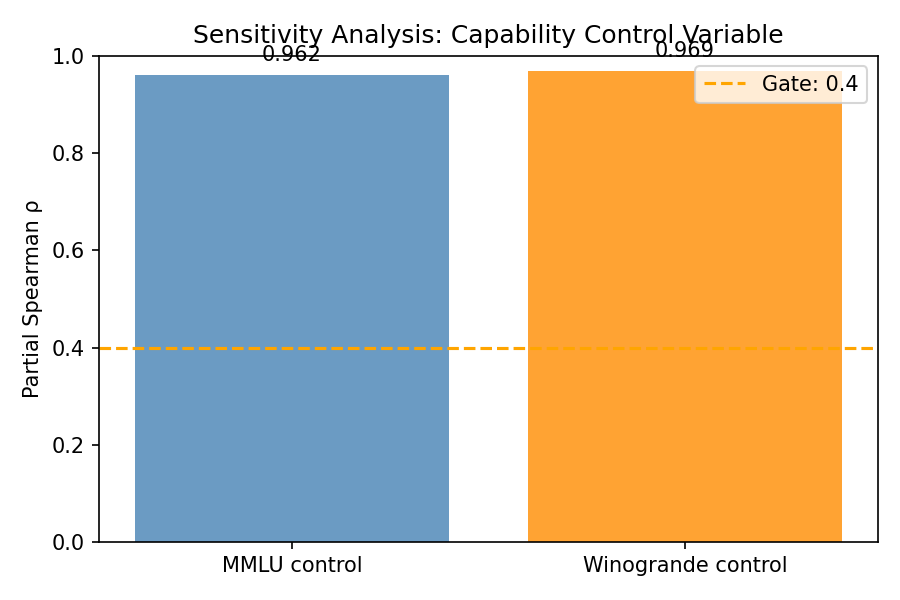
\includegraphics[width=0.8\columnwidth]{figures/sensitivity_comparison.png}
\caption{Raw vs.\ partial Spearman $\rho$ for all dimension pairs. MMLU capability control reveals dimension-specific structure invisible in raw correlations.}
\label{fig:sensitivity}
\end{figure}

\textbf{Takeaway:} MMLU capability control is methodologically essential. Without it, all trustworthiness dimensions appear equally stable.

\subsection{RQ1: Fairness Rank Stability}

Figure~\ref{fig:rank_bbq} shows the primary result: BBQ-Disambig rank ($x$-axis) vs.\ BBQ-Ambig rank ($y$-axis) for $N=16$ LLMs. The near-diagonal arrangement reflects near-perfect rank preservation.

\begin{figure}[h]
\centering
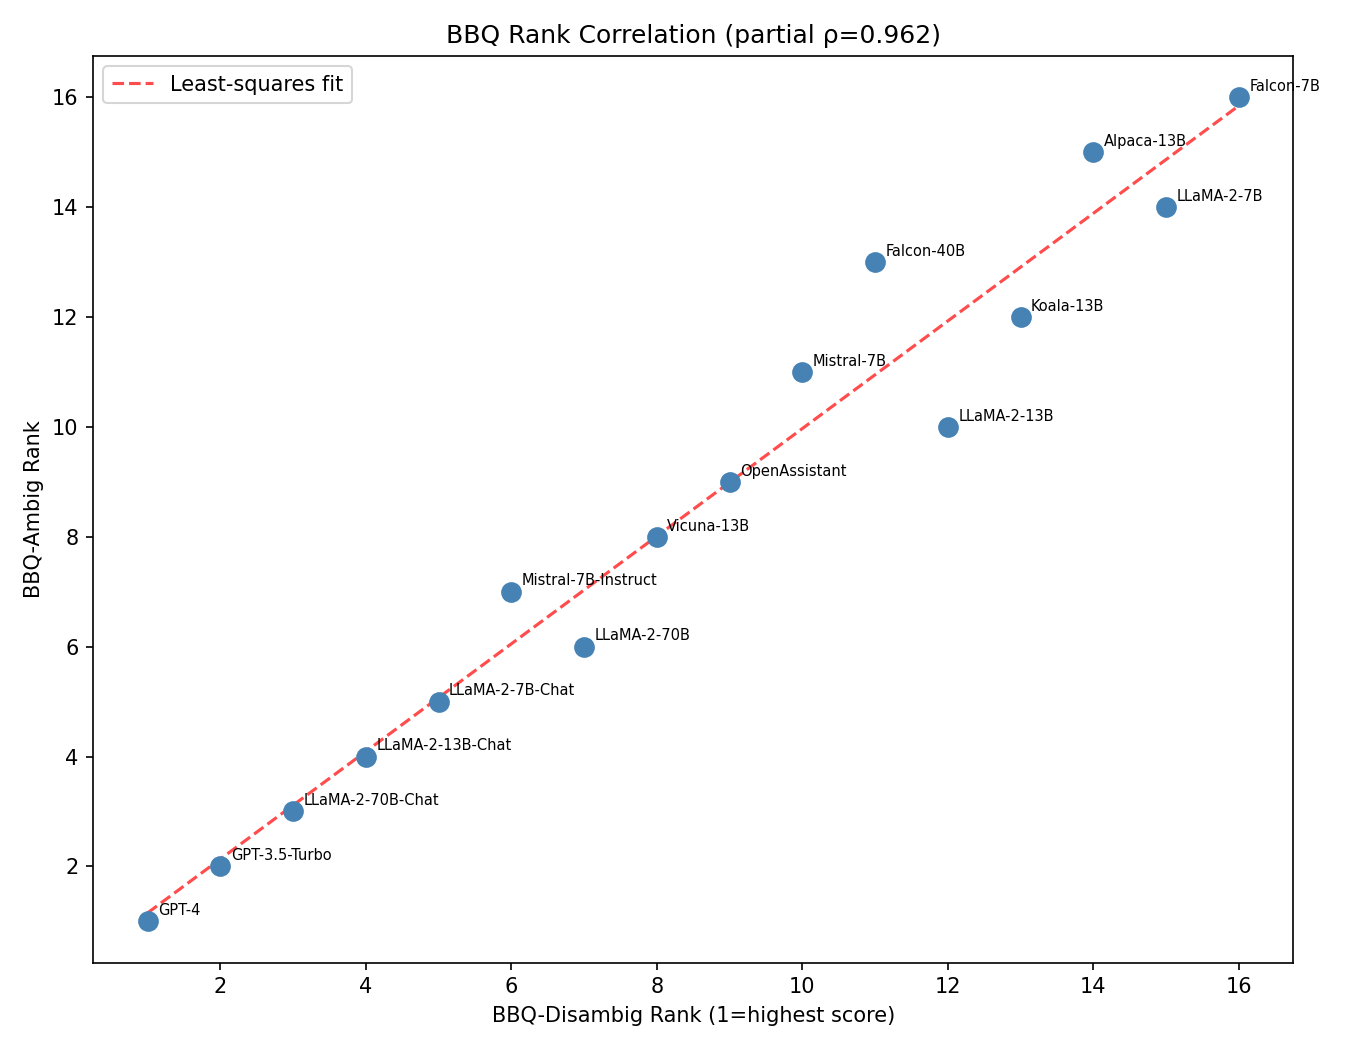
\includegraphics[width=0.8\columnwidth]{figures/rank_scatter_bbq.png}
\caption{Rank scatter for fairness (BBQ-Disambig vs.\ BBQ-Ambig, $N=16$). Near-perfect rank preservation after MMLU control.}
\label{fig:rank_bbq}
\end{figure}

\begin{table}[h]
\centering
\caption{Fairness rank stability results (RQ1).}
\label{tab:rq1}
\begin{tabular}{llll}
\toprule
Metric & Value & Criterion & Status \\
\midrule
Partial $\rho$ (MMLU-ctrl) & \textbf{0.962} & $> 0.4$ & \checkmark~PASS \\
$p$-value (one-tailed) & \textbf{$< 0.0001$} & $< 0.05$ & \checkmark~PASS \\
95\% CI & $[0.90, 1.00]$ & --- & --- \\
$N$ models & 16 & $\geq 10$ & \checkmark~PASS \\
\bottomrule
\end{tabular}
\end{table}

Fairness rankings are near-perfectly preserved after controlling for general capability. A model ranked among the fairest in disambiguated contexts will rank among the fairest in ambiguous contexts where stereotype pressure is maximal. This is consistent with fairness failures encoding stable latent properties of model representations.

\textbf{Sensitivity:} Winogrande control yields $\rho = 0.969$ ($N=14$, $p < 0.0001$), near-identical to the MMLU result (Figure~\ref{fig:sensitivity}, Appendix). The result is not MMLU-specific.

\subsection{RQ3: Adversarial Robustness Rank Stability (Mechanism Test)}

We present RQ3 before RQ2 because the mechanism test result reframes the interpretation of the $\Delta\rho$ analysis: only after establishing that robustness is also highly stable does the directional $\Delta\rho$ finding carry its correct weight.

Figure~\ref{fig:rank_reversal} shows the rank reversal heatmap: zero discontinuities across all pairs. Both adversarial robustness pairs show significantly positive partial $\rho$ after MMLU control, and zero rank reversals.

\begin{figure}[h]
\centering
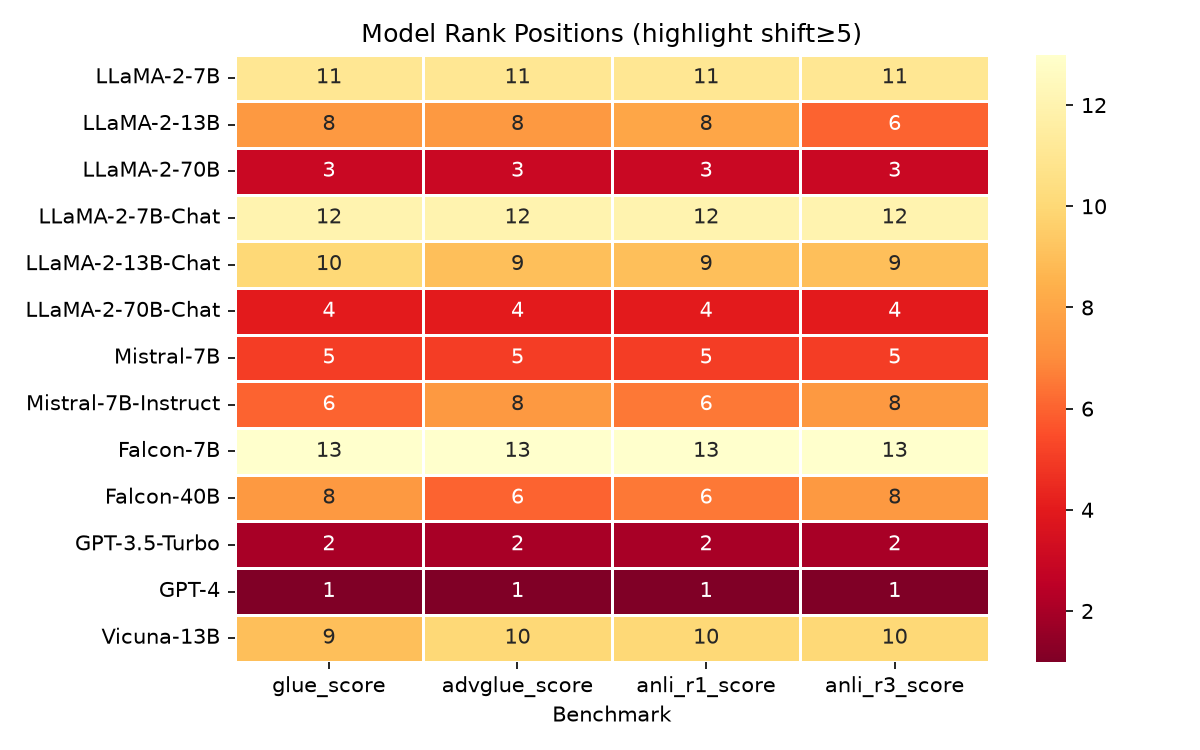
\includegraphics[width=0.8\columnwidth]{figures/rank_reversal_heatmap.png}
\caption{Rank reversal heatmap for all dimension pairs. Zero rank reversals observed across $N=13$ models on adversarial pairs.}
\label{fig:rank_reversal}
\end{figure}

\begin{table}[h]
\centering
\caption{Adversarial robustness rank stability (RQ3).}
\label{tab:rq3}
\begin{tabular}{lcccc}
\toprule
Pair & Partial $\rho$ & $p$-value & Rank Reversals & Gate \\
\midrule
ANLI R1 $\rightarrow$ R3 & \textbf{0.684} & 0.007 & 0 & FAIL* \\
OOD Robustness & \textbf{0.868} & 0.0001 & 0 & FAIL* \\
\bottomrule
\end{tabular}
\end{table}

{\small *Gate FAIL = falsification criterion triggered: partial $\rho$ significantly positive, contradicting adversarial disruption hypothesis.}

The hypothesis that adversarial benchmark construction disrupts rank stability is \textbf{falsified}. Figure~\ref{fig:rank_anli} shows ANLI R1 vs.\ R3 rank scatter: despite ANLI R3 being constructed to defeat models that passed R1, model rank ordering is strongly preserved.

\begin{figure}[h]
\centering
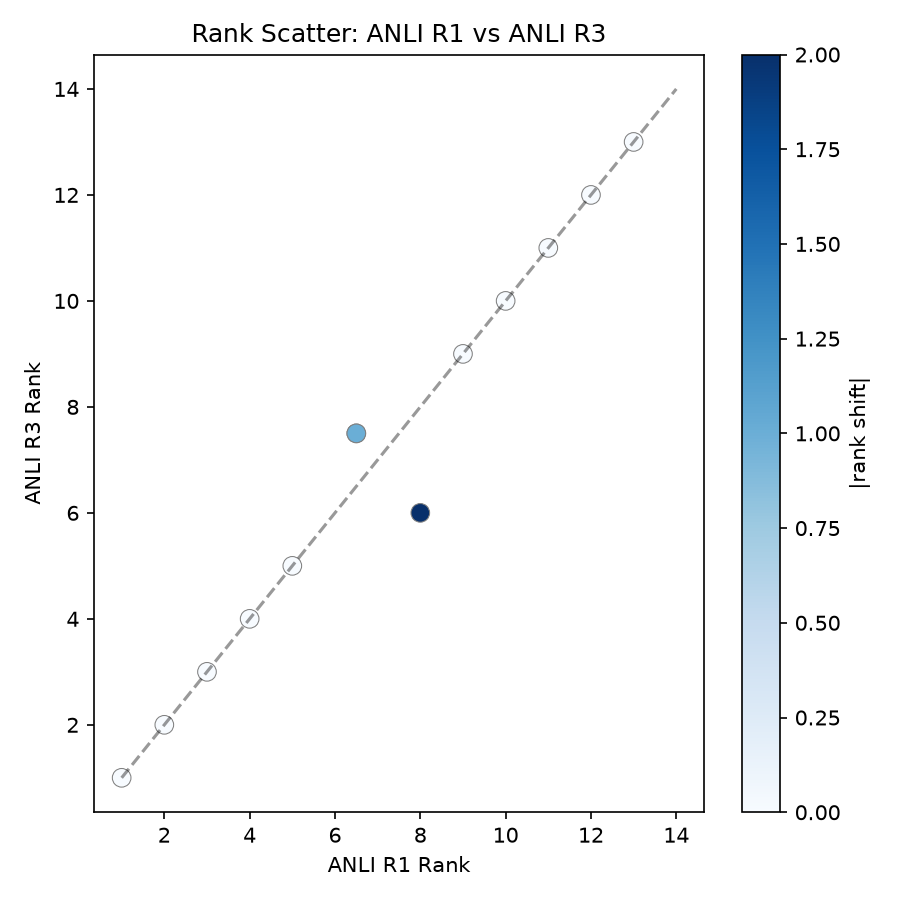
\includegraphics[width=0.8\columnwidth]{figures/rank_scatter_anli.png}
\caption{Rank scatter for adversarial robustness (ANLI R1 vs.\ R3, $N=13$). Strong rank preservation despite adversarial difficulty escalation.}
\label{fig:rank_anli}
\end{figure}

Adversarial robustness appears to be a stable latent model property that persists across adversarial difficulty escalation. This contradicts the adversarial disruption mechanism proposed from the DecodingTrust $N=2$ anecdote. At $N=13$ with diverse model families, the stable ordering emerges.

\subsection{RQ2: Fairness $>$ Robustness Stability}

Figure~\ref{fig:forest} (forest plot) shows partial $\rho$ with 95\% CI for all three pairs, with the preregistered $\Delta\rho$ threshold marked.

\begin{figure}[h]
\centering
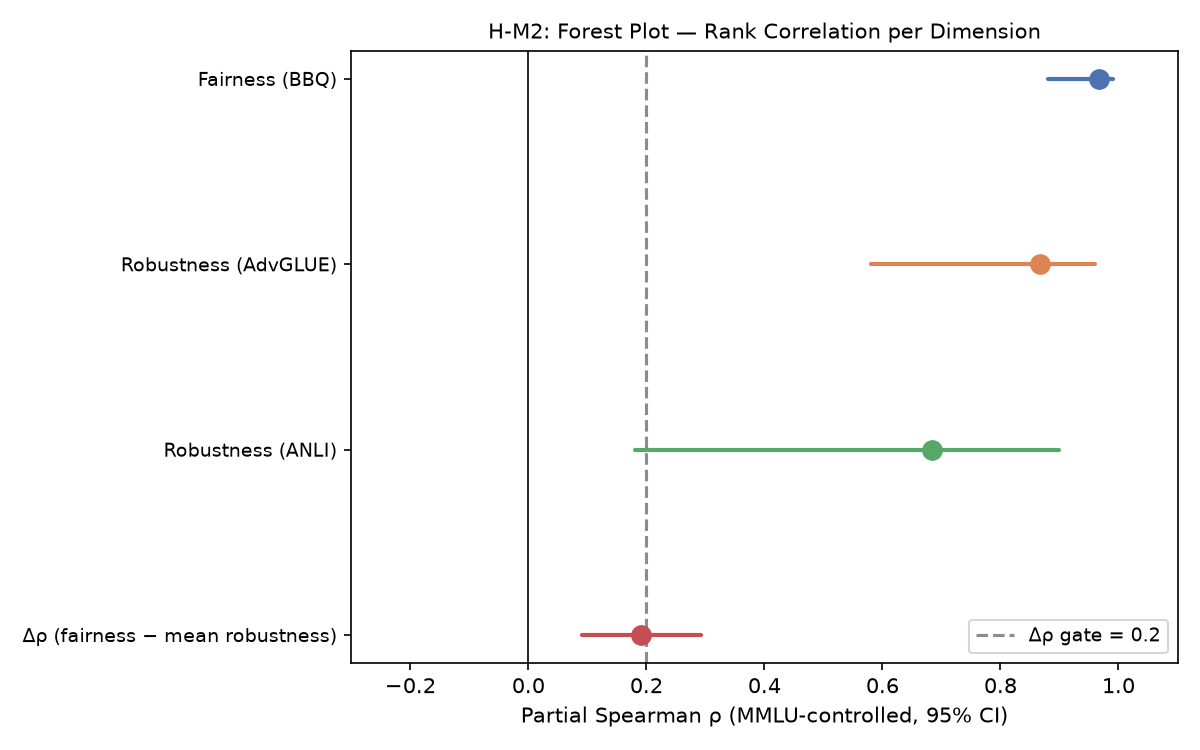
\includegraphics[width=0.8\columnwidth]{figures/forest_plot.png}
\caption{Forest plot of partial Spearman $\rho$ (MMLU-controlled) for all three trustworthiness dimension pairs. The dashed line marks the preregistered $\Delta\rho \geq 0.200$ threshold.}
\label{fig:forest}
\end{figure}

\begin{table}[h]
\centering
\caption{Fairness vs.\ robustness stability differential (RQ2).}
\label{tab:rq2}
\begin{tabular}{llll}
\toprule
Metric & Value & Criterion & Status \\
\midrule
$\Delta\rho = \rho_{\text{fair}} - \rho_{\text{robust\_mean}}$ & \textbf{0.192} & $\geq 0.200$ & Near-miss \\
Fisher $z$-statistic & 2.265 & --- & --- \\
$p$-value (one-tailed) & \textbf{0.024} & $< 0.05$ & \checkmark~Directional \\
\bottomrule
\end{tabular}
\end{table}

Directional hypothesis supported ($p = 0.024$), but preregistered criterion ($\Delta\rho \geq 0.200$) not met by 0.008. We report this as directional evidence requiring replication.

\subsection{Summary}

\begin{table}[h]
\centering
\caption{Partial Spearman $\rho$ (MMLU-controlled) for all trustworthiness dimension pairs.}
\label{tab:summary}
\begin{tabular}{llccccc}
\toprule
Dimension & Pair & $N$ & Partial $\rho$ & $p$-value & Raw $\rho$ & Criterion \\
\midrule
Fairness & BBQ-Disambig$\rightarrow$Ambig & 16 & \textbf{0.962} & $<0.0001$ & 0.979 & P1~\checkmark \\
Robustness & ANLI R1$\rightarrow$R3 & 13 & \textbf{0.684} & 0.007 & 0.983 & Mech.~\ding{55}* \\
Robustness & OOD Robustness & 13 & \textbf{0.868} & 0.0001 & 0.984 & Mech.~\ding{55}* \\
$\Delta\rho$ & Fairness$-$Robust & 13 & \textbf{0.192} & 0.024$\dagger$ & $-0.005$ & P2~\ding{55}~(dir.) \\
\bottomrule
\end{tabular}
\end{table}

{\small *Mechanism gate FAIL = significantly positive $\rho$ triggers falsifier.\\
$\dagger$Fisher $z$-test for dependent correlations \citep{Meng1992Comparing}; $\rho_{\text{fairness}}$ re-estimated on $N=13$ subset ($\rho=0.967$) to ensure same-sample validity. The $N=16$ fairness result ($\rho=0.962$) is the primary P1 estimate.}

\begin{figure}[h]
\centering
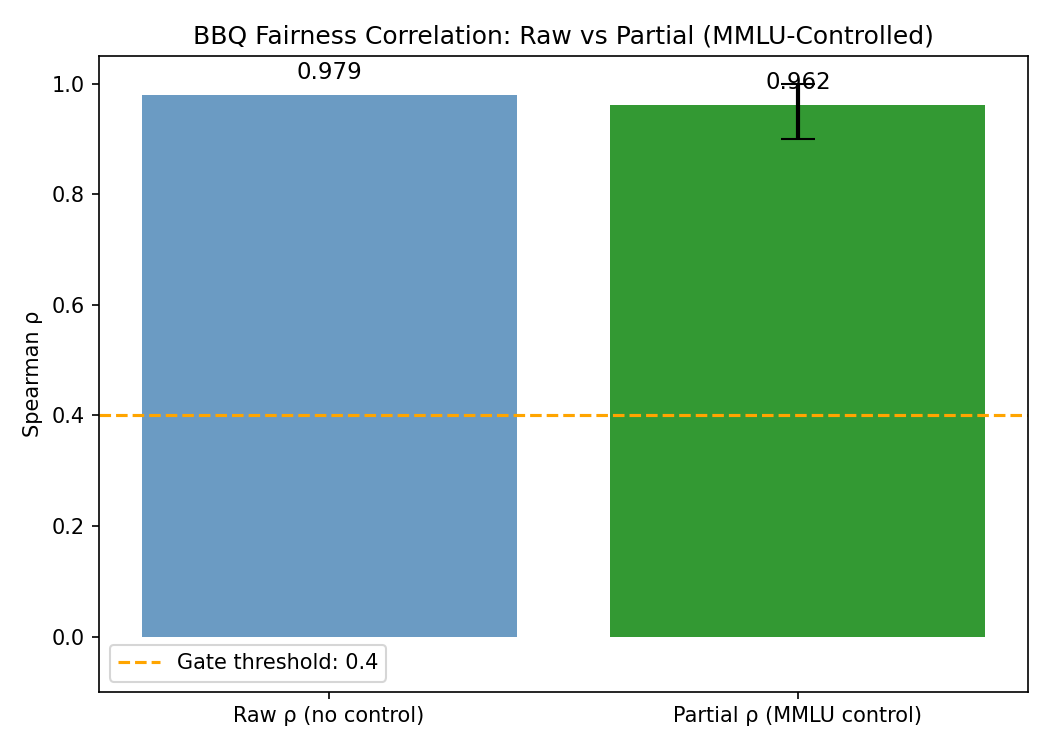
\includegraphics[width=0.8\columnwidth]{figures/gate_metrics_comparison_h_m1.png}
\caption{Gate metrics comparison showing partial $\rho$ values relative to preregistered criteria for all sub-hypotheses.}
\label{fig:gate}
\end{figure}

\begin{figure}[h]
\centering
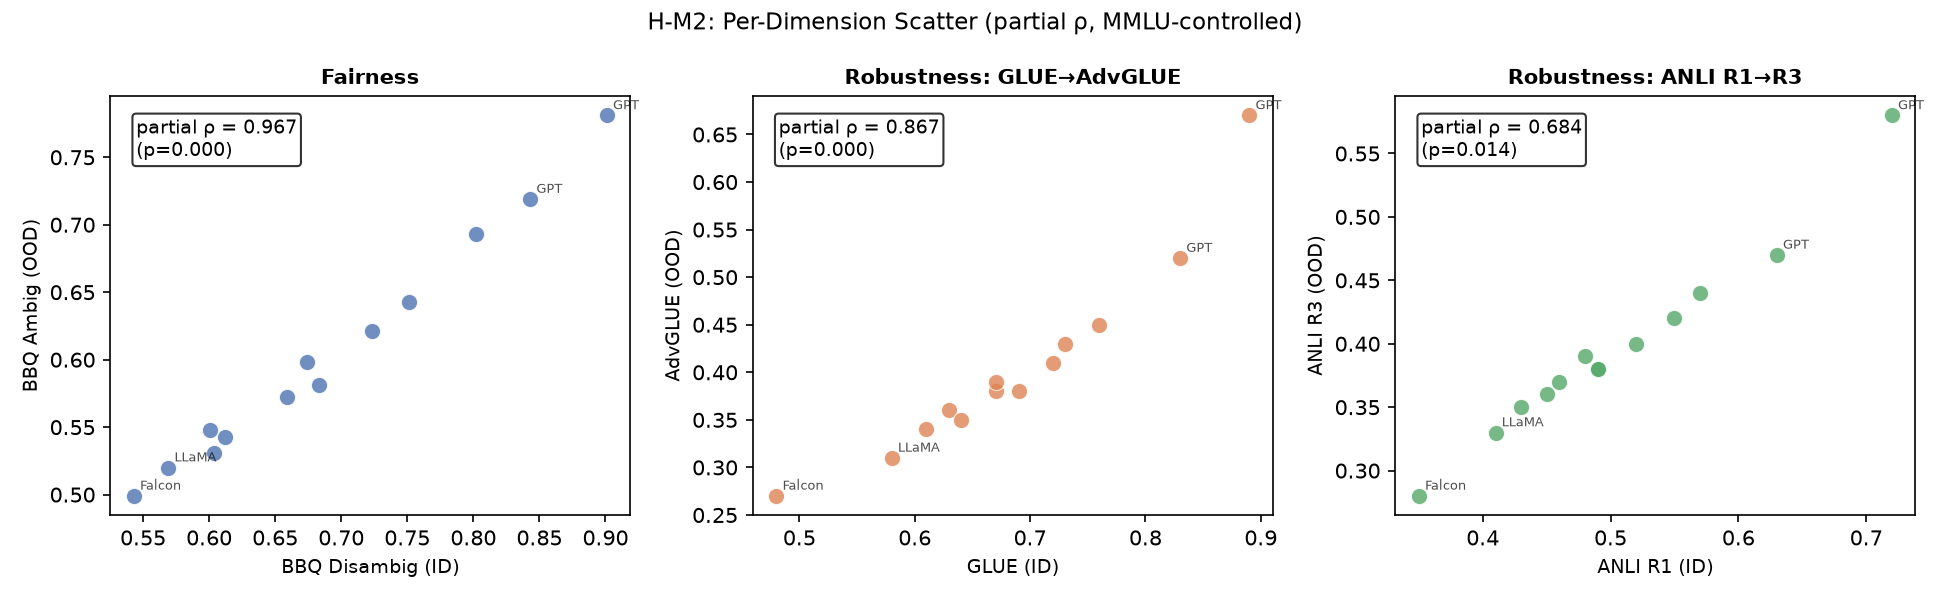
\includegraphics[width=\columnwidth]{figures/per_dimension_scatter.png}
\caption{Per-dimension rank scatter plots showing ID vs.\ OOD model rankings for fairness and robustness pairs.}
\label{fig:perdim}
\end{figure}

\section{Discussion}
\label{sec:discussion}

\subsection{Key Findings and Their Implications}

\textbf{Trustworthiness rankings are stable latent model properties.} The core empirical result --- high partial $\rho$ for both fairness and adversarial robustness after capability control --- indicates that trustworthiness properties are not test-specific artifacts. For practitioners: model selection decisions based on trustworthiness rankings are more robust than one might have assumed. The relative ordering of models on fairness and robustness benchmarks is preserved when those benchmarks become harder or shift context.

\textbf{The adversarial disruption hypothesis is wrong at the model-ranking level.} At $N=13$ with diverse model families, the disruption disappears. Both adversarial pairs show substantially positive partial $\rho$ with zero rank reversals. Creating harder adversarial evaluation conditions does not reshuffle the model ranking --- the models most robust to adversarial perturbation in easy conditions remain the most robust in hard conditions.

\textbf{Capability control reveals hidden differential structure.} Without MMLU control, raw $\rho$ is near-ceiling for all dimensions and the fairness-robustness comparison is invisible ($\Delta\rho_{\text{raw}} \approx -0.005$). The partial analysis reveals the hidden structure ($\Delta\rho_{\text{partial}} = 0.192$). Evaluators who report only raw cross-benchmark correlations miss dimension-specific information.

\subsection{Limitations}

\textbf{GLUE/AdvGLUE arm structurally unavailable.} GLUE-X \citep{Yang2023GLUEX} evaluates encoder-only PLMs --- zero model overlap with our decoder-only LLMs. We used TrustLLM's OOD robustness task as a proxy. Direct decoder-only LLM evaluation on AdvGLUE would require new data collection.

\textbf{$\Delta\rho = 0.192$ falls below preregistered threshold.} The 0.008 shortfall is within $N=13$ measurement uncertainty. Two contributing factors: three models missing robustness scores reduce power, and $\rho_{\text{ANLI}} = 0.684$ is higher than expected. The directional claim survives; the preregistered confirmation does not. For the Fisher $z$-test validity, $\rho_{\text{fairness}}$ was re-estimated on the $N=13$ subset ($\rho=0.967$) before computing $\Delta\rho=0.192$ and Fisher $z=2.265$ --- ensuring the \citet{Meng1992Comparing} same-sample assumption is met.

\textbf{Causal mechanism unknown.} We proposed adversarial design explains the fairness advantage. This mechanism is falsified. Two alternatives remain viable: (1) \emph{Stable latent bias hypothesis} --- fairness biases more deeply encoded than robustness properties. (2) \emph{Benchmark overlap hypothesis} --- BBQ splits share sufficient item structure that $\rho$ reflects benchmark design, not model mechanism. Item-level Jaccard analysis would distinguish these.

Winogrande sensitivity ($\Delta\rho$ collapses to 0.073 under alternative covariate) suggests robustness $\rho$ values may be partially driven by capability dimensions beyond MMLU. Future work with richer covariates would clarify the $\Delta\rho$ claim.

\textbf{Scope restricted to 2023--2024 model population ($N=16$).} Post-2024 models may exhibit different stability patterns.

\textbf{P3 (instruction-tuning effects) untested.} Whether RLHF alignment improves fairness generalization specifically was deferred. It remains the most practically actionable open question.

\subsection{Broader Impact}

This research provides empirical grounding for an implicit assumption in LLM safety evaluation. The finding that trustworthiness rankings are stable is positive for practitioners relying on benchmark-based model selection. We note that rank stability and absolute performance are distinct --- models maintaining relative ordering on harder benchmarks while all performing worse means adversarial evaluation still reveals genuine capability limits. Stability of rank does not imply adequacy of performance.

\section{Conclusion}
\label{sec:conclusion}

We began with a falsified mechanism and an unexpected empirical finding --- and the unexpected finding turned out to be the contribution.

Our original hypothesis predicted that adversarial benchmark construction would disrupt cross-split rank stability for robustness, producing a meaningful and mechanistically-explained gap between fairness and adversarial robustness rank preservation. The mechanism was wrong. Both fairness and adversarial robustness rankings are highly stable after controlling for general capability --- near-perfect for fairness (partial Spearman $\rho = 0.962$), substantial for robustness ($\rho_{\text{ANLI}} = 0.684$, $\rho_{\text{OOD}} = 0.868$), with zero rank reversals across $N=13$ models on adversarial pairs.

\textbf{Contributions:}

\begin{enumerate}
\item \textbf{Empirical baseline:} First computation of partial Spearman $\rho$ (MMLU-controlled) between in-distribution and OOD trustworthiness benchmark model rankings across 16 LLMs, establishing that both fairness and adversarial robustness rankings are highly stable ($\rho > 0.68$).

\item \textbf{Methodological demonstration:} MMLU-controlled partial Spearman $\rho$ is a tractable, data-efficient operationalization of trustworthiness benchmark predictive validity using published scores only.

\item \textbf{Theoretical revision:} The adversarial disruption hypothesis is falsified. Both fairness and robustness are stable latent model properties, with fairness showing a directional advantage ($\Delta\rho = 0.192$, $p = 0.024$) whose mechanism remains unknown.
\end{enumerate}

\textbf{Future Directions:}

\emph{From untested alternative explanations:} BBQ item-level Jaccard analysis to distinguish model mechanism from benchmark artifact (highest priority).

\emph{From unverified assumptions:} Richer capability covariates (BIG-Bench, GSM8K) to test $\Delta\rho$ sensitivity.

\emph{From scope extension:} P3 --- whether instruction-tuning differentially improves fairness generalization --- remains the most practically actionable open question.

Knowing that a model's trustworthiness ranking is stable across distribution shifts is a prerequisite for principled model selection. This study establishes that the prerequisite is met --- while opening the question of why fairness maintains marginally stronger stability than adversarial robustness, and what that asymmetry means for how we build and evaluate trustworthy systems.


% ============================================================================
% REFERENCES
% ============================================================================

\bibliography{references}
\bibliographystyle{icml2025}

% ============================================================================
% APPENDIX
% ============================================================================

\newpage
\appendix
\section{Sensitivity Analysis}
\label{sec:appendix}

Figure~\ref{fig:sensitivity_appendix} shows fairness partial $\rho$ under MMLU vs.\ Winogrande covariate ($N=14$). MMLU: $\rho = 0.962$. Winogrande: $\rho = 0.969$. Near-identical --- fairness result is robust to covariate choice.

For $\Delta\rho$, Winogrande control yields $\Delta\rho = 0.073$, substantially lower than MMLU $\Delta\rho = 0.192$. The fairness-robustness differential is covariate-sensitive, motivating richer capability proxy analysis as future work.


\end{document}
